\begin{figure}[htbp]
\centering
% Thesis-wide categorical color palette
% Usage: % Thesis-wide categorical color palette
% Usage: % Thesis-wide categorical color palette
% Usage: \input{figures/palette} in any figure file
%
% Muted primary colors -- print-friendly, visually distinct.
% Inspired by Cooper Union's red/blue primaries, softened for
% academic figures. Use palA-palC for data series in scatter
% plots, line charts, bar charts, etc.

\definecolor{palA}{HTML}{1F77B4}   % Tableau blue
\definecolor{palB}{HTML}{D62728}   % Tableau red
\definecolor{palC}{HTML}{2CA02C}   % Tableau green
 in any figure file
%
% Muted primary colors -- print-friendly, visually distinct.
% Inspired by Cooper Union's red/blue primaries, softened for
% academic figures. Use palA-palC for data series in scatter
% plots, line charts, bar charts, etc.

\definecolor{palA}{HTML}{1F77B4}   % Tableau blue
\definecolor{palB}{HTML}{D62728}   % Tableau red
\definecolor{palC}{HTML}{2CA02C}   % Tableau green
 in any figure file
%
% Muted primary colors -- print-friendly, visually distinct.
% Inspired by Cooper Union's red/blue primaries, softened for
% academic figures. Use palA-palC for data series in scatter
% plots, line charts, bar charts, etc.

\definecolor{palA}{HTML}{1F77B4}   % Tableau blue
\definecolor{palB}{HTML}{D62728}   % Tableau red
\definecolor{palC}{HTML}{2CA02C}   % Tableau green

\definecolor{encfade}{HTML}{B8D2E6}
\definecolor{outfront}{HTML}{DCE8F4}
\definecolor{outtop}{HTML}{EBF1F8}
\definecolor{outside}{HTML}{C2D6E8}
\definecolor{fcfront}{HTML}{B3CEE4}
\definecolor{fctop}{HTML}{CDDEF0}
\definecolor{fcside}{HTML}{8DB3D2}
\definecolor{sslfront}{HTML}{B8D8A0}
\definecolor{ssltop}{HTML}{CBE4B8}
\definecolor{sslside}{HTML}{8FB870}

\newcommand{\cuboid}[7]{%
    \fill[#5, draw=black!35, line join=round]
        (#1, {-#3/2}, 0) -- ({#1+#2}, {-#3/2}, 0) --
        ({#1+#2}, {#3/2}, 0) -- (#1, {#3/2}, 0) -- cycle;
    \fill[#6, draw=black!35, line join=round]
        (#1, {#3/2}, 0) -- ({#1+#2}, {#3/2}, 0) --
        ({#1+#2}, {#3/2}, #4) -- (#1, {#3/2}, #4) -- cycle;
    \fill[#7, draw=black!35, line join=round]
        ({#1+#2}, {-#3/2}, 0) -- ({#1+#2}, {#3/2}, 0) --
        ({#1+#2}, {#3/2}, #4) -- ({#1+#2}, {-#3/2}, #4) -- cycle;
}

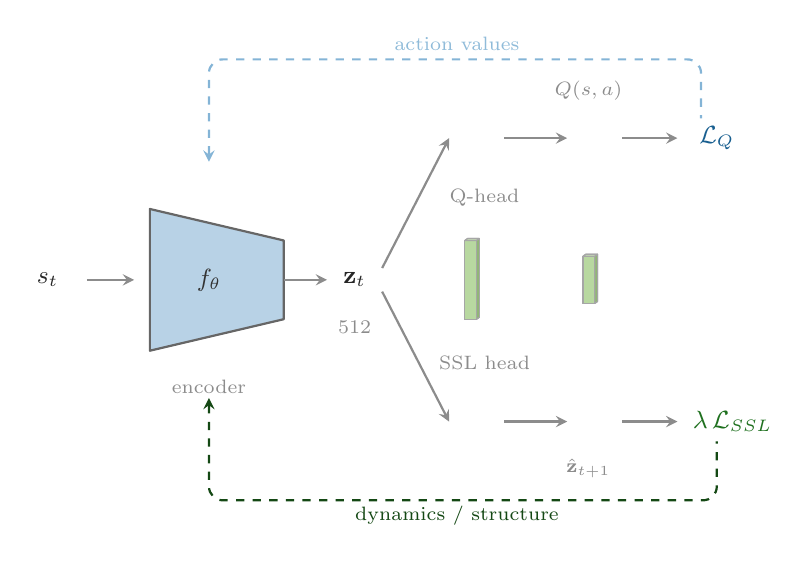
\begin{tikzpicture}[
    x={(1cm,0cm)}, y={(0cm,1cm)}, z={(0.35cm,0.25cm)},
    arr/.style={->, thick, >=stealth, black!45},
    gradarr/.style={<-, thick, >=stealth, dashed},
    lbl/.style={font=\scriptsize, text=black!45},
]

% Observation label
\node[font=\small, text=black!85] at (-0.5, 0, 0) {$s_t$};
\draw[arr] (0.0, 0, 0) -- (0.6, 0, 0);

% Encoder (trapezoid)
\fill[encfade, draw=black!60, thick, line join=round]
    (0.8, -0.9, 0) -- (0.8, 0.9, 0) -- (2.5, 0.5, 0)
    -- (2.5, -0.5, 0) -- cycle;
\node[font=\small, text=black!80] at (1.55, 0, 0) {$f_\theta$};

% z_t label
\node[font=\small, text=black!85] (zt) at (3.4, 0, 0)
    {$\mathbf{z}_t$};
\draw[arr] (2.5, 0, 0) -- (3.05, 0, 0);

% === Upper path: Q-head ===
\draw[arr] (3.75, 0.15, 0) -- (4.6, 1.8, 0);

% FC layer (upper)
\cuboid{4.8}{0.15}{1.0}{0.1}{fcfront}{fctop}{fcside}
\draw[arr] (5.3, 1.8, 0) -- (6.1, 1.8, 0);

% Q-values output (upper)
\cuboid{6.3}{0.15}{0.6}{0.1}{outfront}{outtop}{outside}
\node[lbl, anchor=south] at (6.37, 2.15, 0) {$Q(s,a)$};

% Q loss
\draw[arr] (6.8, 1.8, 0) -- (7.5, 1.8, 0);
\node[font=\small, text=palA!80!black] at (8.0, 1.8, 0)
    {$\mathcal{L}_{\text{Q}}$};

% Q-head label (between fork and cuboids)
\node[lbl] at (5.05, 1.05, 0) {Q-head};

% === Lower path: SSL head ===
\draw[arr] (3.75, -0.15, 0) -- (4.6, -1.8, 0);

% SSL projection (lower, green cuboid)
\cuboid{4.8}{0.15}{1.0}{0.1}{sslfront}{ssltop}{sslside}
\draw[arr] (5.3, -1.8, 0) -- (6.1, -1.8, 0);

% SSL output (lower, green cuboid)
\cuboid{6.3}{0.15}{0.6}{0.1}{sslfront}{ssltop}{sslside}
\node[lbl, anchor=north] at (6.37, -2.15, 0)
    {$\hat{\mathbf{z}}_{t+1}$};

% SSL loss
\draw[arr] (6.8, -1.8, 0) -- (7.5, -1.8, 0);
\node[font=\small, text=palC!70!black] at (8.2, -1.8, 0)
    {$\lambda\,\mathcal{L}_{\text{SSL}}$};

% SSL-head label
\node[lbl] at (5.05, -1.05, 0) {SSL head};

% Encoder + bottleneck labels
\node[lbl, anchor=north] at (1.55, -1.15, 0) {encoder};
\node[lbl, anchor=north] at (3.4, -0.4, 0) {512};

% === Gradient arrows (colored to show which loss) ===
% Q gradient (blue, above)
\draw[gradarr, palA!55, rounded corners=5pt]
    (1.55, 1.5, 0) -- (1.55, 2.8, 0) -- (7.8, 2.8, 0)
    -- (7.8, 2.05, 0);
\node[lbl, text=palA!50] at (4.7, 3.0, 0) {action values};

% SSL gradient (green, below)
\draw[gradarr, palC!45!black, rounded corners=5pt]
    (1.55, -1.5, 0) -- (1.55, -2.8, 0) -- (8.0, -2.8, 0)
    -- (8.0, -2.05, 0);
\node[lbl, text=palC!45!black] at (4.7, -3.0, 0)
    {dynamics / structure};

\end{tikzpicture}
\caption{Dual-objective training. Self-supervised learning adds a
  second path: the encoder receives gradients from both
  $\mathcal{L}_{\text{Q}}$ (action values) and
  $\lambda\mathcal{L}_{\text{SSL}}$ (dynamics), shaping its
  representations with complementary signals.}
\label{fig:dual-objective}
\end{figure}
